\documentclass[aspectratio=169]{beamer}

\usetheme{HGF}

\usepackage{amsmath}
\usepackage{caption}
\usepackage[utf8x]{inputenc}
\usepackage{graphicx}
\usepackage{pgfplots}
\usepackage{textcomp}
\usepackage{tikz}
\usepackage{xcolor}
\usepackage{xmpmulti}
\usepackage{xpatch}

\xpatchcmd{\itemize}
{\def\makelabel}
{\ifnum\@itemdepth=1\relax
    \setlength\itemsep{2ex}% separation for first level
    \else
    \ifnum\@itemdepth=2\relax
    \setlength\itemsep{1ex}% separation for second level
    \else
    \ifnum\@itemdepth=3\relax
    \setlength\itemsep{0.5ex}% separation for third level
    \fi\fi\fi\def\makelabel
}
{}
{}

\usetikzlibrary{
    decorations, 
    shapes,
    shapes.misc
}
\tikzset{cross/.style={path picture={ 
    \draw[black](path picture bounding box.south east) -- (path picture bounding box.north west) (path picture bounding box.south west) -- (path picture bounding box.north east);
}}}

\pgfplotsset{compat=newest}

\graphicspath{{./images/}}
\makeatletter
\def\input@path{{./}{./images}}
\makeatother

\newcommand\imageright[1]{ %
    \caption*{\scalebox{.5}{\textcolor{lightgray}{\textcopyright~#1}}} %
}

\DeclareMathOperator*{\argmin}{arg\,min}

\title{Machine Learning with Neural Networks}
\subtitle{GridKa School 2018}
\author{Markus Götz}
\date{2018-08-29}
\institute{KIT}

\begin{document}
    
\section{Introduction}
\label{sec:introduction}

\maketitle

%%%%%%%%%%%%%%%%%%%%%%%%%%%%%%%%%%%%%%%%%%%%%%%%%%%%%%%%%%%%%%%%%%%%%%%%%%%
\begin{frame}
\frametitle{Outline}
    \tableofcontents[hideallsubsections]
\end{frame}

\section{Machine Learning Fundamentals}
\label{sec:machine-learning}

\subsection{Terminology}
\label{subsec:terminology}

\begin{frame}
\frametitle{Terminology}
\begin{columns}
    \begin{column}{0.48\textwidth}
        \begin{itemize}
            \item \textbf{Samples} or instances,\\ 
            individual observations in your data,\\
            e.g. an image, a specimen
            \item \textbf{Features} or attributes,\\ 
            single characteristic of a sample,\\
             e.g. a pixel, measured weight
            \item \textbf{Channels} or time,\\
            depth information,\\
            color channels, change over time
        \end{itemize}
    \end{column}
    \begin{column}{0.48\textwidth}
        \begin{figure}
            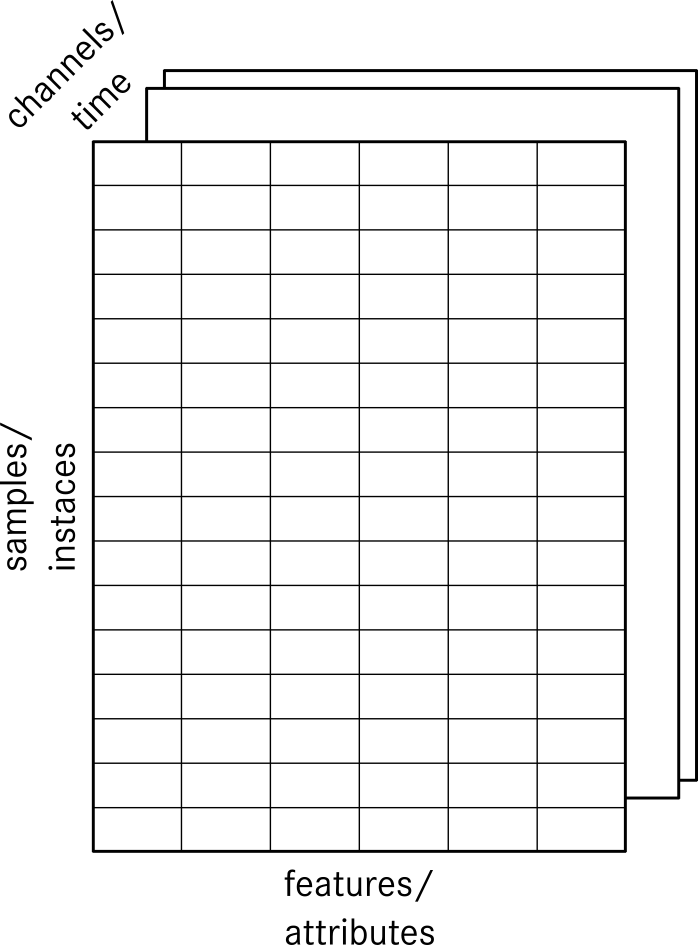
\includegraphics{terminology.png}
        \end{figure}
    \end{column}
\end{columns}
\end{frame}

\begin{frame}
    \frametitle{Terminology}
    
    \begin{figure}
        \centering
        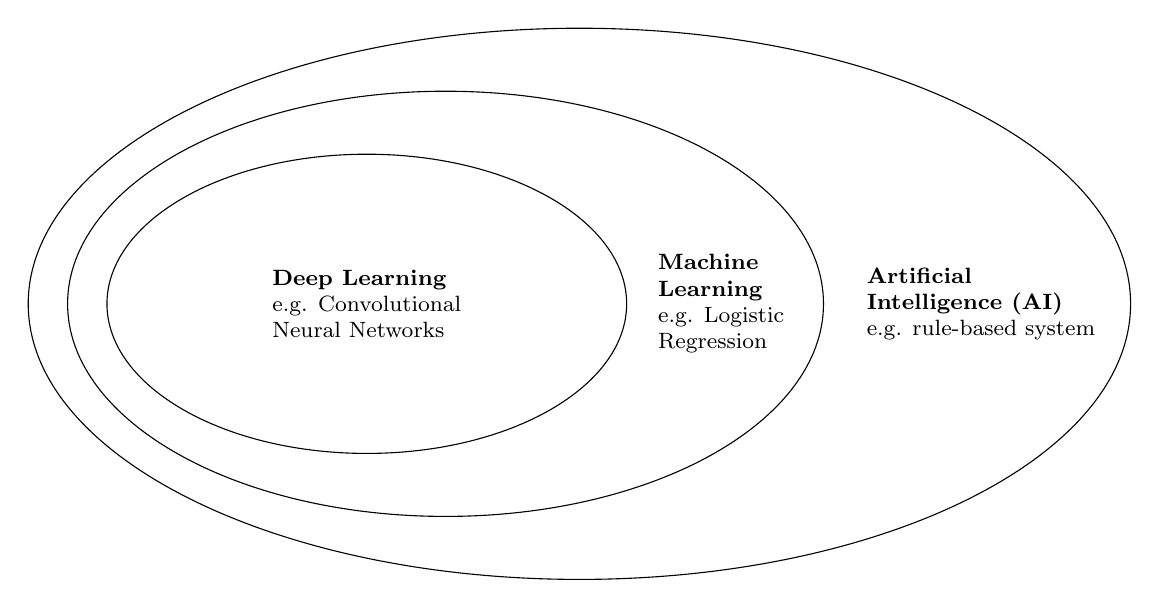
\begin{tikzpicture}[fill=white, font=\footnotesize]
            \draw (0, 0) ellipse (7.0 and 3.5);
            \node[align=left] at (5.1, 0.0) {\textbf{Artificial}\\ \textbf{Intelligence (AI)}\\e.g. rule-based system};
            
            \draw (-1.7, 0) ellipse (4.8 and 2.7) (1.8, 0.0) node[align=left] {\textbf{Machine}\\ \textbf{Learning}\\ e.g. Logistic\\ Regression};
            
            \draw (-2.7, 0) ellipse (3.3 and 1.9) (-2.7, 0.0) node[align=left] {\textbf{Deep Learning}\\ e.g. Convolutional\\ Neural Networks};
        \end{tikzpicture}
    \end{figure}
\end{frame}

\begin{frame}
\frametitle{Why now?}
    \begin{itemize}
        \item \textbf{Technology revolution}---vector processors (e.g. GPGPUs), auto-gradient software
        \item \textbf{Data availability}---large, partially freely available, collections of labeled data
        \item \textbf{Mathematical advances}---latest addition, investigation of new model elements, e.g. activation functions, normalization
    \end{itemize}
\end{frame}

\begin{frame}
\frametitle{Learning Approaches}
    \begin{itemize}
        \item \textbf{Supervised learning:} Learn by ``mimicking supervisor'', i.e. pattern annotations\\ 
        examples: image classification, stock forecasting
        \item \textbf{Unsupervised learning:} Determine patterns purely based on data\\ examples: customer cluster analysis, distribution estimation
        \item \textbf{Reinforcement learning:} Pavlov-style learning with punishment and reward in dynamic environments\\
        examples: game AIs, e.g. AlphaGo or Dota OpenAI
    \end{itemize}
\end{frame}

\begin{frame}
\frametitle{Notation Disclaimer}
\begin{itemize}
    \item \textbf{Small letters:} vectors or matrices, e.g. $x$ or $y$
    \item \textbf{Hats:} predictions or estimates, e.g. $\hat{y}$
    \item \textbf{Indices:} elements of vectors and matrices, e.g. $x_{i}$
\end{itemize}

\medskip
\end{frame}

\begin{frame}
\frametitle{Linear Regression}
    \begin{columns}
        \begin{column}{0.43\textwidth}
            \begin{figure}
                \begin{tikzpicture}
                    \begin{axis}[
                        width=\linewidth, 
                        grid=both,
                        grid style={line width=.3pt, draw=blue!10},
                        major grid style={line width=.3pt, draw=blue!10},
                        minor tick num=3,
                        xlabel={$x$},
                        ylabel={$y$}, 
                        ticks=none,
                        axis x line=center,
                        axis y line=center,
                        xmin=-0.1,
                        xmax=3.0,
                        ymin=-0.1,
                        ymax=1.6
                    ]
                    \only<1->{\addplot [blue, only marks, mark size=1pt] coordinates {
                        (0.3, 0.10054215032765762)
                        (0.4263157894736842, 0.12363160260273953)
                        (0.5526315789473685, 0.2228985962683488)
                        (0.6789473684210527, 0.32110283680834006)
                        (0.8052631578947369, 0.3464254484709207)
                        (0.9315789473684213, 0.530973472751518)
                        (1.0578947368421054, 0.508700039361571)
                        (1.1842105263157896, 0.5115642913251457)
                        (1.310526315789474, 0.6517708510332498)
                        (1.4368421052631581, 0.7372626388813315)
                        (1.5631578947368425, 0.7555802030144961)
                        (1.6894736842105267, 0.8020873099226213)
                        (1.8157894736842108, 0.920859494738636)
                        (1.9421052631578952, 0.9025123937365214)
                        (2.0684210526315794, 1.0124087289206862)
                        (2.1947368421052635, 1.081906810760111)
                        (2.3210526315789477, 1.089021024213448)
                        (2.447368421052632, 1.3056222105270976)
                        (2.573684210526316, 1.2573605236570795)
                        (2.7, 1.2546989788028189)
                    };}
                    \node<1-> at (axis cs:1.8,0.5) [blue] {\footnotesize\emph{data}};
                    
                    \only<2->{\addplot [red, thick, mark=none] {0.5*x};}
                    \node<2-> at (axis cs:2.0,1.3) [red] {\footnotesize\emph{model}};
                    \end{axis} 
                \end{tikzpicture}
            \end{figure}
        \end{column}
        \begin{column}{0.53\textwidth}
            \begin{itemize}
                \item<1-> \textbf{Data set:} $\{samples, labels\}=\{x, y\}$
                \item<2-> \textbf{Model:} definition $\hat{y}=wx+b$\\ with $w$ and $b$ trainable parameters
                \item<3-> \textbf{Loss function:} or cost/objective\\
                $J(w,b)=MSE(w,b)=\frac{1}{N}\sum_{i=1}^{N}(y_i-\hat{y_i})^2$
                \item<4-> \textbf{Train:} the model, e.g. optimization\\
                $\hat{w}, \hat{b}=\argmin J(w, b)$ \\
                
            \end{itemize}
        \end{column}
    \end{columns}

    \bigskip
    \begin{itemize}
        \item<5>
            \begin{center}
                \textbf{Basic recipe for most machine learning algorithms}
            \end{center}
    \end{itemize}
\end{frame}

\begin{frame}
\frametitle{Optimization: Gradient Descent}

\begin{itemize}
    \item Iterative optimization technique, weight update in direction of negative gradient
\end{itemize}
\begin{center}$w_{i+1}=w_{i}-lr\nabla_{w_{i}}J(w)$\end{center}
\vspace{-0.7cm}
\begin{columns}
    \begin{column}{0.48\textwidth}
        \begin{figure}
            \begin{tikzpicture}
            \begin{axis}[
                width=\linewidth,
                height=0.6\textheight, 
                grid=both,
                grid style={line width=.3pt, draw=blue!10},
                major grid style={line width=.3pt, draw=blue!10},
                minor tick num=3,
                xlabel={$x$},
                ylabel={$y$}, 
                ticks=none,
                axis x line=center,
                axis y line=center,
                xmin=-0.1,
                xmax=3.0,
                ymin=-0.1,
                ymax=1.6
            ]
            
            \addplot [red, thick, mark=none, dashed, domain=0:4] {0.1*(x - 1.5) + 0.75};
            \node at (axis cs:0.3,0.7) [red] {\footnotesize$w_{1}$};
            \addplot [red, thick, mark=none, dashed, domain=0:4] {0.25*(x - 1.5) + 0.75)};
            \node at (axis cs:0.3,0.35) [red] {\footnotesize$w_{2}$};
            \addplot [red, thick, mark=none] {0.5*x};
            \node at (axis cs:2.2,1.3) [red] {\footnotesize$w_{s}$};
            
            
            \addplot [blue, only marks, mark size=1pt] coordinates {
                (0.3, 0.10054215032765762)
                (0.4263157894736842, 0.12363160260273953)
                (0.5526315789473685, 0.2228985962683488)
                (0.6789473684210527, 0.32110283680834006)
                (0.8052631578947369, 0.3464254484709207)
                (0.9315789473684213, 0.530973472751518)
                (1.0578947368421054, 0.508700039361571)
                (1.1842105263157896, 0.5115642913251457)
                (1.310526315789474, 0.6517708510332498)
                (1.4368421052631581, 0.7372626388813315)
                (1.5631578947368425, 0.7555802030144961)
                (1.6894736842105267, 0.8020873099226213)
                (1.8157894736842108, 0.920859494738636)
                (1.9421052631578952, 0.9025123937365214)
                (2.0684210526315794, 1.0124087289206862)
                (2.1947368421052635, 1.081906810760111)
                (2.3210526315789477, 1.089021024213448)
                (2.447368421052632, 1.3056222105270976)
                (2.573684210526316, 1.2573605236570795)
                (2.7, 1.2546989788028189)
            };
            \node at (axis cs:1.8,0.5) [blue] {\footnotesize\emph{data}};
            \end{axis} 
            \end{tikzpicture}
        \end{figure}
    \end{column}
    \begin{column}{0.48\textwidth}
        \begin{figure}
            
\begin{tikzpicture}
            \begin{axis}[
            width=\linewidth, 
            height=0.6\textheight, 
            grid=both,
            grid style={line width=.3pt, draw=blue!10},
            major grid style={line width=.3pt, draw=blue!10},
            minor tick num=3,
            xlabel={$w$},
            ylabel={$J$}, 
            ticks=none,
            axis x line=center,
            axis y line=center,
            xmin=-0.1,
            xmax=3.0,
            ymin=-0.1,
            ymax=1.6
            ]
            % domain=0.25:2.75
            \addplot [black, thick, mark=none, smooth, samples=50, domain=0.3:2.7] {0.9*(x-1.5)^2 + 0.2};
            \addplot [red, only marks, mark size=2pt] coordinates {
                (1.5, 0.2)
                (1.0, 0.425)
                (0.5, 1.1)
            };
            \addplot [red, mark=none] coordinates {
                (1.5, 0.05)
                (1.5, 0.15)
            };
            \addplot [red, mark=none] coordinates {
                (1.0, 0.05)
                (1.0, 0.37)
            };
            \addplot [red, mark=none] coordinates {
                (0.5, 0.05)
                (0.5, 1.00)
            };
            \addplot [blue, mark=none] coordinates {
                (0.53, 0.95)
                (0.53, 0.43)
                (0.93, 0.43)
            };
            \draw [->, red](axis cs:0.57,1.07)--(axis cs:0.98,0.48);
            \node at (axis cs:1.20,0.8) [blue] {$lr\frac{dJ}{dw}$};
            \node at (axis cs:0.7,0.1) [red] {\footnotesize$w_{1}$};
            \node at (axis cs:1.2,0.1) [red] {\footnotesize$w_{2}$};
            \node at (axis cs:1.7,0.1) [red] {\footnotesize$w_{s}$};
            \end{axis} 
            \end{tikzpicture}
        \end{figure}
    \end{column}
\end{columns}
\begin{itemize}
    \item $lr$ is learning rate, gradient update factor
    \item \textbf{Stochastic gradient descent (SGD)}, sample subset (\textbf{batch}) updates
\end{itemize}
\end{frame}

\begin{frame}
\frametitle{Bias Trick}

\begin{itemize}
\item Cumbersome to keep track of weights $w$ and bias $b$
\item \textbf{Idea:} fuse both into single weight matrix

\begin{alignat*}{11}
\hat{y}&=&w&x&+b&\leftrightarrow&\hat{y}&=&w&x \\
\hat{y}&=&\begin{pmatrix}
w_{1} \\
w_{2} \\
\vdots \\
w_{n}
\end{pmatrix}'&
\begin{pmatrix}
x_{i,1}\\
x_{i,2}\\
\vdots\\
x_{i,n}\\
\end{pmatrix}&+b&\leftrightarrow&\hat{y}&=&
\begin{pmatrix}
\textbf{b} \\
w_{1} \\
w_{2} \\
\vdots \\
w_{n}
\end{pmatrix}'&
\begin{pmatrix}
\textbf{1}\\
x_{i,1}\\
x_{i,2}\\
\vdots\\
x_{i,n}\\
\end{pmatrix}
\end{alignat*}
\end{itemize}
\end{frame}

\subsection{Logistic Regression}
\label{subsec:logistic-regression}

\begin{frame}
\frametitle{Pattern Recognition Types}
    \begin{columns}
        \begin{column}{0.48\textwidth}
            \begin{itemize}
                \item \textbf{Regression:} predict continuous value, e.g. stock price, $y\in\mathbb{R}$
                \item \textbf{Classification:} assign sample to a category, e.g. ``spam''/``no spam''\\special form of regression,\\ where $y$ in fixed interval
            \end{itemize}
        \end{column}
        \begin{column}{0.48\textwidth}
            \begin{figure}
                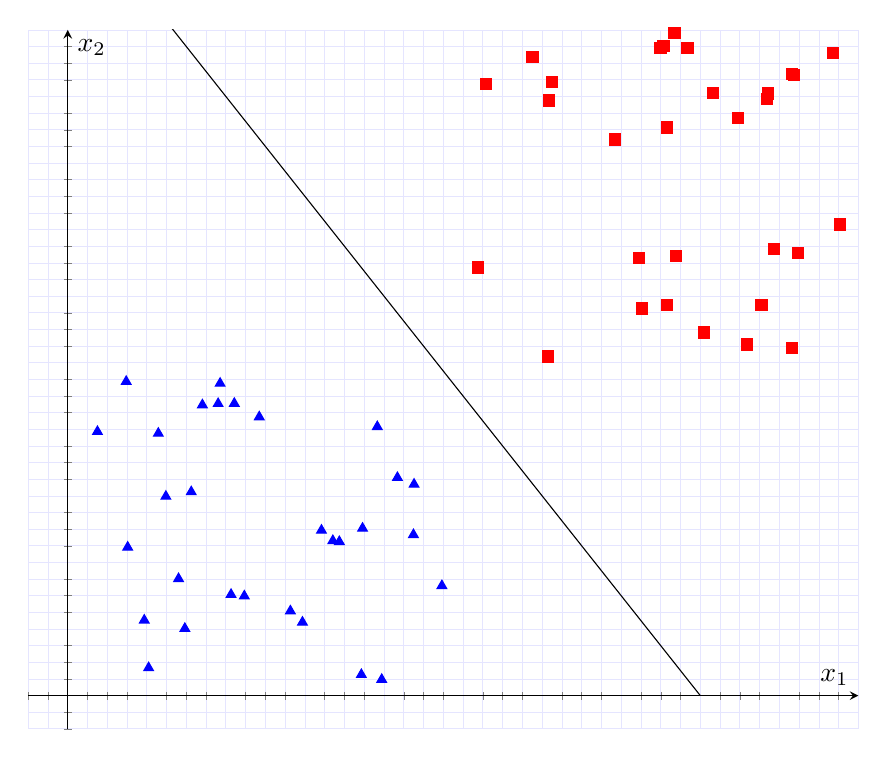
\begin{tikzpicture}
                \begin{axis}[
                    width=\linewidth, 
                    grid=both,
                    grid style={line width=.3pt, draw=blue!10},
                    major grid style={line width=.3pt, draw=blue!10},
                    minor tick num=3,
                    xlabel={$x_1$},
                    ylabel={$x_2$}, 
                    ticks=none,
                    axis x line=center,
                    axis y line=center,
                    xmin=-0.1,
                    xmax=2.0,
                    ymin=-0.1,
                    ymax=2.0
                ]
                \addplot [blue, only marks, mark size=2pt, mark=triangle*] coordinates {
                    (0.3405210822112612, 0.8733467370280228)
                    (0.6417180817230281, 0.4966306166288442)
                    (0.31236861944953176, 0.6121119482760103)
                    (0.4843845705001969, 0.8372723451578254)
                    (0.6705319198897809, 0.46544265493212356)
                    (0.15159623290041857, 0.44576239992026545)
                    (0.9463452893119627, 0.33010610736211987)
                    (0.19348743132666624, 0.22660283230073164)
                    (0.2961562717918107, 0.20157698331379592)
                    (0.38534371092248065, 0.9381135102799997)
                    (0.0750871559631675, 0.7932733927855736)
                    (0.14786222142469718, 0.9437344260840296)
                    (0.5936565086474459, 0.22034859139209484)
                    (0.22907523223663817, 0.7878697366360873)
                    (0.794139162809545, 0.048334139863450254)
                    (0.2481683008839609, 0.5986112990477678)
                    (0.28024639511041294, 0.35123819610592255)
                    (0.7426502500585584, 0.06302390692215687)
                    (0.4465644429635456, 0.29914396434886015)
                    (0.7829307093180131, 0.8078686578775368)
                    (0.38036767570222685, 0.8771510877252888)
                    (0.5630903124576907, 0.2542147707582497)
                    (0.8338634277199973, 0.6550543205600249)
                    (0.8759184599366046, 0.6349455271372683)
                    (0.6869371856928128, 0.46250259195124)
                    (0.4212924892722074, 0.8777507521988864)
                    (0.874384938038331, 0.4834185999120415)
                    (0.2045721844969517, 0.0834946363978849)
                    (0.41302308334280347, 0.30372338532728305)
                    (0.7456467692023212, 0.5026216907475388)
                };
                \addplot [red, only marks, mark size=2pt, mark=square*] coordinates {
                    (1.7706837759950487, 1.808884456339976)
                    (1.6097673166601565, 1.0910700963071096)
                    (1.8311427531366666, 1.043397970524071)
                    (1.7686274677101825, 1.7929387383883477)
                    (1.8476473528536392, 1.3287310154974328)
                    (1.51561309479197, 1.7071106254688428)
                    (1.4441136349948995, 1.3151875726875542)
                    (1.6320240433560618, 1.8106133358232555)
                    (1.93615150297599, 1.9318761344130344)
                    (1.6957150249499564, 1.7353082711966865)
                    (1.3832499009666868, 1.6706984272443974)
                    (1.5390778241411607, 1.3212483573991296)
                    (1.5067423770579214, 1.951642819491536)
                    (1.5162449533753577, 1.1744133372978611)
                    (1.452290644909902, 1.1628763191277276)
                    (1.215300195996602, 1.0190784373594854)
                    (1.832559930658315, 1.8667682767915506)
                    (1.7174600650559508, 1.0548065370692519)
                    (1.2178766103535255, 1.7877897361036623)
                    (1.5675863098843703, 1.946616980060258)
                    (1.9539865940177632, 1.415630588037017)
                    (1.0386711055996827, 1.28647932022736)
                    (1.4994662399845793, 1.9459071761746531)
                    (1.057157101434958, 1.8380166331031762)
                    (1.7853872352436764, 1.3426683001589166)
                    (1.75459402308149, 1.1746356610150874)
                    (1.534515821721585, 1.990233613715762)
                    (1.8364540007603098, 1.863869583052054)
                    (1.2251698093011876, 1.8446796325215797)
                    (1.1756480589317504, 1.9193842816924964)
                };
                \addplot [black, mark=none, domain=0:1.6] {-1.5*x+2.4};
                \end{axis}
                \end{tikzpicture}
            \end{figure}
        \end{column}
    \end{columns}
\end{frame}

\begin{frame}
\frametitle{Logistic Regression}

\begin{columns}
    \begin{column}{0.48\textwidth}
        \begin{figure}
            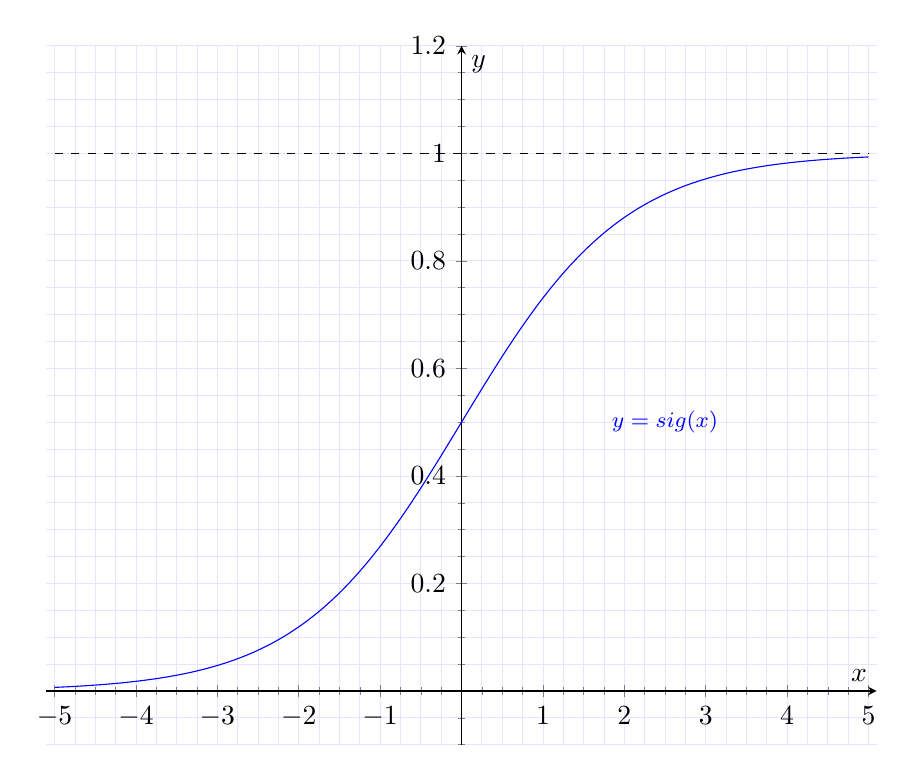
\begin{tikzpicture}
            \begin{axis}[
                width=\linewidth, 
                grid=both,
                grid style={line width=.3pt, draw=blue!10},
                major grid style={line width=.3pt, draw=blue!10},
                minor tick num=3,
                xlabel={$x$},
                ylabel={$y$}, 
                axis x line=center,
                axis y line=center,
                xmin=-5.1,
                xmax=5.1,
                ymin=-0.1,
                ymax=1.2
            ]
            \addplot [blue, mark=none, smooth, samples=50] {1/(1 + e^-x)};
            \addplot [black, dashed, mark=none] {1};
            \node at (axis cs:2.5,0.5) [blue] {\footnotesize$y=sig(x)$};
            \end{axis}
            \end{tikzpicture}
        \end{figure}
    \end{column}
    \begin{column}{0.48\textwidth}
        \begin{itemize}
            \item Squash linear regression output in fixed interval, e.g. $y\in[0,1]$
            \item Interpretation: \textbf{probability} of sample belonging to a binary class
            \item \textbf{sigmoid-/logistic} function: $sig(z)=\frac{1}{1+e^{-x}}$
            \item \textbf{Model:} $h=sig(wx)=\frac{1}{1+e^{-wx}}$
            \item \textbf{Prediction:} $\hat{y}=1$ if $h\geq 0.5$\\\hspace{2.15cm}$\hat{y}=0$ if $h<0.5$
        \end{itemize}
    \end{column}
\end{columns}
\end{frame}

\begin{frame}
\frametitle{Logistic Regression}
\begin{columns}
    \begin{column}{0.48\textwidth}
        \begin{itemize}
            \item \textbf{Data set} must be mapped
            \begin{itemize}
                \item \tikz{\node[fill=red, rectangle ,minimum width=0.2cm,minimum height=0.2cm,inner sep=0pt] at (0,0) {};} $\rightarrow 0$
                \item \tikz{\node[fill=blue, isosceles triangle,isosceles triangle stretches,shape border rotate=90,minimum width=0.2cm,minimum height=0.2cm,inner sep=0pt] at (0,0) {};} $\rightarrow 1$
            \end{itemize}
            \item \textbf{Model:} $h=sig(wx)=\frac{1}{1+e^{-wx}}$
            \item \textbf{Loss function:} $J(w)=MSE(w)=(y-\hat{y})^2$\\
            \medskip
            $\frac{dJ}{dw}=(\hat{y}-y)*(\hat{y}-\hat{y}^2)*x$
            \item \textbf{Train:} gradient descent optimization
        \end{itemize}
    \end{column}
    \begin{column}{0.48\textwidth}
        \begin{figure}
            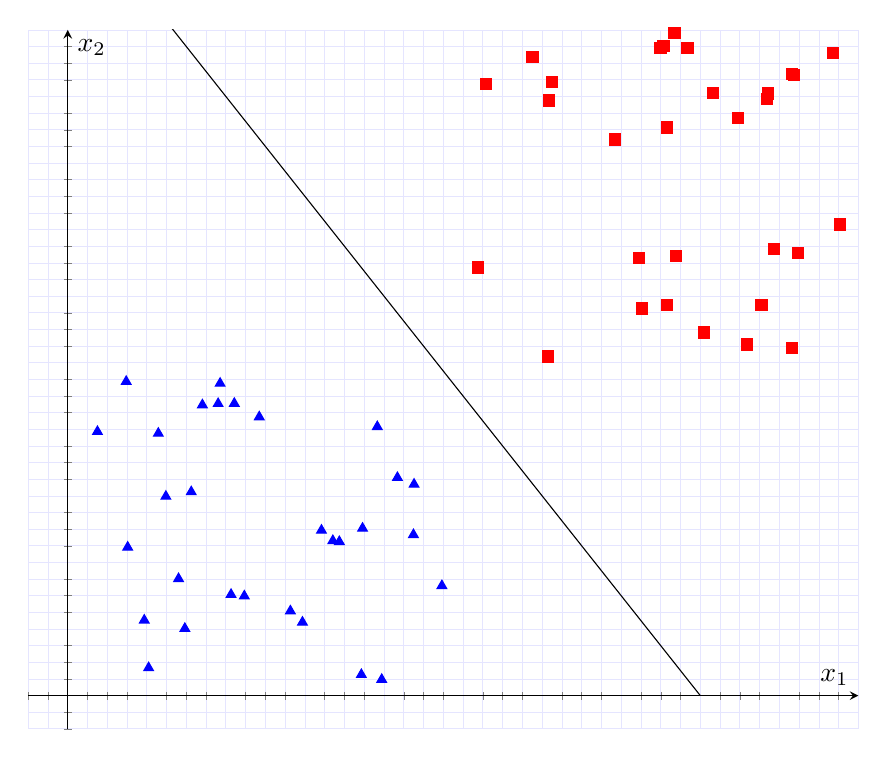
\begin{tikzpicture}
            \begin{axis}[
                width=\linewidth, 
                grid=both,
                grid style={line width=.3pt, draw=blue!10},
                major grid style={line width=.3pt, draw=blue!10},
                minor tick num=3,
                xlabel={$x_1$},
                ylabel={$x_2$}, 
                ticks=none,
                axis x line=center,
                axis y line=center,
                xmin=-0.1,
                xmax=2.0,
                ymin=-0.1,
                ymax=2.0
            ]
            \addplot [blue, only marks, mark size=2pt, mark=triangle*] coordinates {
                (0.3405210822112612, 0.8733467370280228)
                (0.6417180817230281, 0.4966306166288442)
                (0.31236861944953176, 0.6121119482760103)
                (0.4843845705001969, 0.8372723451578254)
                (0.6705319198897809, 0.46544265493212356)
                (0.15159623290041857, 0.44576239992026545)
                (0.9463452893119627, 0.33010610736211987)
                (0.19348743132666624, 0.22660283230073164)
                (0.2961562717918107, 0.20157698331379592)
                (0.38534371092248065, 0.9381135102799997)
                (0.0750871559631675, 0.7932733927855736)
                (0.14786222142469718, 0.9437344260840296)
                (0.5936565086474459, 0.22034859139209484)
                (0.22907523223663817, 0.7878697366360873)
                (0.794139162809545, 0.048334139863450254)
                (0.2481683008839609, 0.5986112990477678)
                (0.28024639511041294, 0.35123819610592255)
                (0.7426502500585584, 0.06302390692215687)
                (0.4465644429635456, 0.29914396434886015)
                (0.7829307093180131, 0.8078686578775368)
                (0.38036767570222685, 0.8771510877252888)
                (0.5630903124576907, 0.2542147707582497)
                (0.8338634277199973, 0.6550543205600249)
                (0.8759184599366046, 0.6349455271372683)
                (0.6869371856928128, 0.46250259195124)
                (0.4212924892722074, 0.8777507521988864)
                (0.874384938038331, 0.4834185999120415)
                (0.2045721844969517, 0.0834946363978849)
                (0.41302308334280347, 0.30372338532728305)
                (0.7456467692023212, 0.5026216907475388)
            };
            \addplot [red, only marks, mark size=2pt, mark=square*] coordinates {
                (1.7706837759950487, 1.808884456339976)
                (1.6097673166601565, 1.0910700963071096)
                (1.8311427531366666, 1.043397970524071)
                (1.7686274677101825, 1.7929387383883477)
                (1.8476473528536392, 1.3287310154974328)
                (1.51561309479197, 1.7071106254688428)
                (1.4441136349948995, 1.3151875726875542)
                (1.6320240433560618, 1.8106133358232555)
                (1.93615150297599, 1.9318761344130344)
                (1.6957150249499564, 1.7353082711966865)
                (1.3832499009666868, 1.6706984272443974)
                (1.5390778241411607, 1.3212483573991296)
                (1.5067423770579214, 1.951642819491536)
                (1.5162449533753577, 1.1744133372978611)
                (1.452290644909902, 1.1628763191277276)
                (1.215300195996602, 1.0190784373594854)
                (1.832559930658315, 1.8667682767915506)
                (1.7174600650559508, 1.0548065370692519)
                (1.2178766103535255, 1.7877897361036623)
                (1.5675863098843703, 1.946616980060258)
                (1.9539865940177632, 1.415630588037017)
                (1.0386711055996827, 1.28647932022736)
                (1.4994662399845793, 1.9459071761746531)
                (1.057157101434958, 1.8380166331031762)
                (1.7853872352436764, 1.3426683001589166)
                (1.75459402308149, 1.1746356610150874)
                (1.534515821721585, 1.990233613715762)
                (1.8364540007603098, 1.863869583052054)
                (1.2251698093011876, 1.8446796325215797)
                (1.1756480589317504, 1.9193842816924964)
            };
            \addplot [black, mark=none, domain=0:1.6] {-1.5*x+2.4};
            \end{axis}
            \end{tikzpicture}
        \end{figure}
    \end{column}
\end{columns}
\end{frame}

\begin{frame}
\frametitle{Computer Vision}
\end{frame}

\begin{frame}
\frametitle{MNIST Dataset}
\end{frame}

\subsection{Libraries}
\label{subsec:libraries}

\subsection{Exercise: Logistic Regression}
\label{subsec:exercise-logistic-regression}

\begin{frame}
    \frametitle{Exercise: Logistic Regression}
    \begin{figure}
        \centering
        \begin{tikzpicture}[]
        \node [inner sep=0pt,above right] { %
            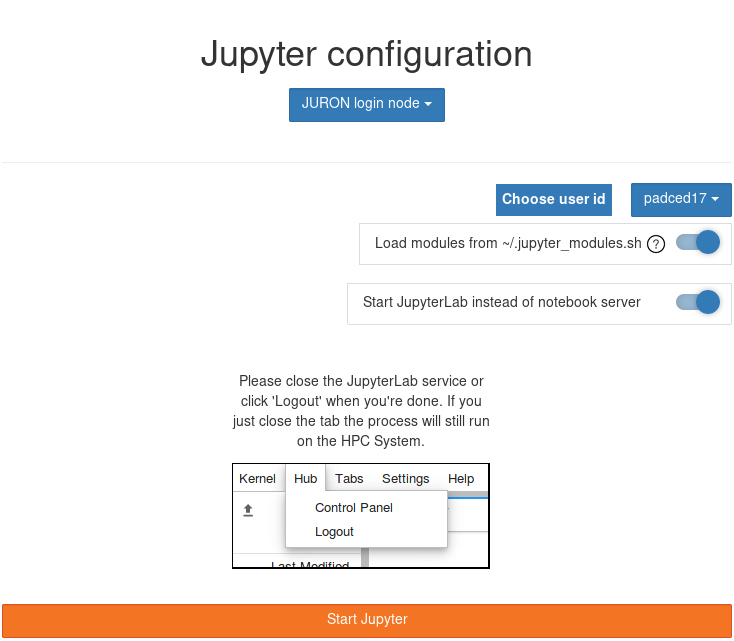
\includegraphics[width=0.5\linewidth]{jupyter.png} %
        };
        % show origin
        \draw [line width=0.6mm, red] (7.05, 4.05) ellipse (0.5 and 0.25);
        \end{tikzpicture}
    \end{figure}
\end{frame}

\begin{frame}
\frametitle{Exercise: Logistic Regression}

\begin{columns}
    \begin{column}{0.48\textwidth}
        \begin{itemize}
            \item \textbf{Data set} must be mapped
            \begin{itemize}
                \item \tikz{\node[fill=red, rectangle ,minimum width=0.2cm,minimum height=0.2cm,inner sep=0pt] at (0,0) {};} $\rightarrow 0$
                \item \tikz{\node[fill=blue, isosceles triangle,isosceles triangle stretches,shape border rotate=90,minimum width=0.2cm,minimum height=0.2cm,inner sep=0pt] at (0,0) {};} $\rightarrow 1$
            \end{itemize}
            \item \textbf{Model:} $h=sig(wx)=\frac{1}{1+e^{-wx}}$
            \item \textbf{Loss function:} $J(w)=MSE(w)=(y-\hat{y})^2$\\
            \medskip
            $\frac{dJ}{dw}=(\hat{y}-y)*(\hat{y}-\hat{y}^2)*x$
            \item \textbf{Train:} $w_{i+1}=w_{i}-lr\frac{dJ}{dw}$
        \end{itemize}
    \end{column}
    \begin{column}{0.48\textwidth}
        \begin{figure}
            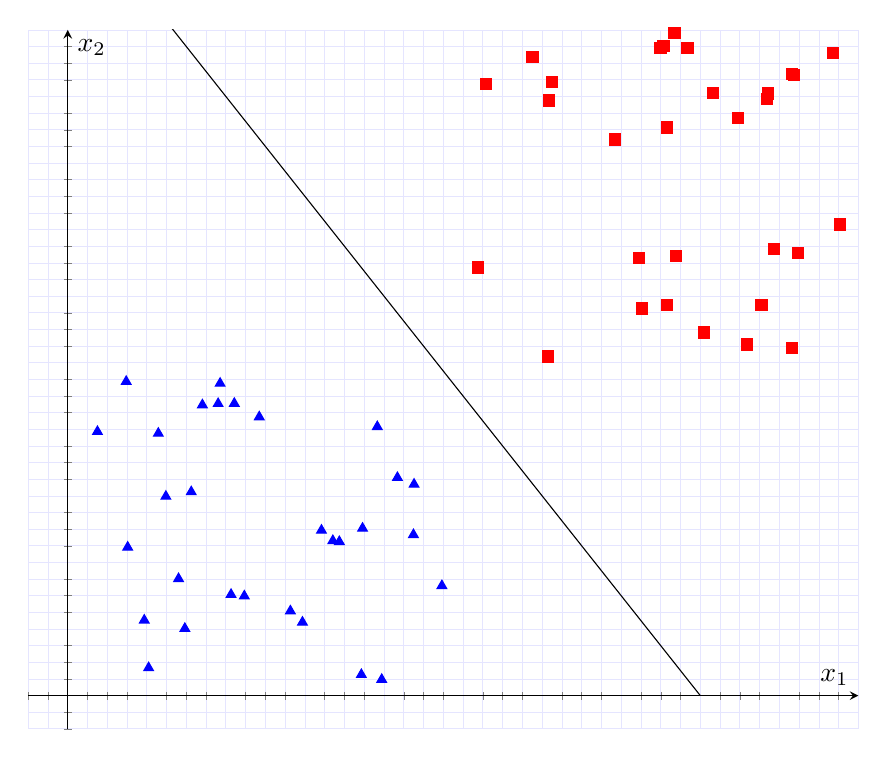
\begin{tikzpicture}
            \begin{axis}[
            width=\linewidth, 
            grid=both,
            grid style={line width=.3pt, draw=blue!10},
            major grid style={line width=.3pt, draw=blue!10},
            minor tick num=3,
            xlabel={$x_1$},
            ylabel={$x_2$}, 
            ticks=none,
            axis x line=center,
            axis y line=center,
            xmin=-0.1,
            xmax=2.0,
            ymin=-0.1,
            ymax=2.0
            ]
            \addplot [blue, only marks, mark size=2pt, mark=triangle*] coordinates {
                (0.3405210822112612, 0.8733467370280228)
                (0.6417180817230281, 0.4966306166288442)
                (0.31236861944953176, 0.6121119482760103)
                (0.4843845705001969, 0.8372723451578254)
                (0.6705319198897809, 0.46544265493212356)
                (0.15159623290041857, 0.44576239992026545)
                (0.9463452893119627, 0.33010610736211987)
                (0.19348743132666624, 0.22660283230073164)
                (0.2961562717918107, 0.20157698331379592)
                (0.38534371092248065, 0.9381135102799997)
                (0.0750871559631675, 0.7932733927855736)
                (0.14786222142469718, 0.9437344260840296)
                (0.5936565086474459, 0.22034859139209484)
                (0.22907523223663817, 0.7878697366360873)
                (0.794139162809545, 0.048334139863450254)
                (0.2481683008839609, 0.5986112990477678)
                (0.28024639511041294, 0.35123819610592255)
                (0.7426502500585584, 0.06302390692215687)
                (0.4465644429635456, 0.29914396434886015)
                (0.7829307093180131, 0.8078686578775368)
                (0.38036767570222685, 0.8771510877252888)
                (0.5630903124576907, 0.2542147707582497)
                (0.8338634277199973, 0.6550543205600249)
                (0.8759184599366046, 0.6349455271372683)
                (0.6869371856928128, 0.46250259195124)
                (0.4212924892722074, 0.8777507521988864)
                (0.874384938038331, 0.4834185999120415)
                (0.2045721844969517, 0.0834946363978849)
                (0.41302308334280347, 0.30372338532728305)
                (0.7456467692023212, 0.5026216907475388)
            };
            \addplot [red, only marks, mark size=2pt, mark=square*] coordinates {
                (1.7706837759950487, 1.808884456339976)
                (1.6097673166601565, 1.0910700963071096)
                (1.8311427531366666, 1.043397970524071)
                (1.7686274677101825, 1.7929387383883477)
                (1.8476473528536392, 1.3287310154974328)
                (1.51561309479197, 1.7071106254688428)
                (1.4441136349948995, 1.3151875726875542)
                (1.6320240433560618, 1.8106133358232555)
                (1.93615150297599, 1.9318761344130344)
                (1.6957150249499564, 1.7353082711966865)
                (1.3832499009666868, 1.6706984272443974)
                (1.5390778241411607, 1.3212483573991296)
                (1.5067423770579214, 1.951642819491536)
                (1.5162449533753577, 1.1744133372978611)
                (1.452290644909902, 1.1628763191277276)
                (1.215300195996602, 1.0190784373594854)
                (1.832559930658315, 1.8667682767915506)
                (1.7174600650559508, 1.0548065370692519)
                (1.2178766103535255, 1.7877897361036623)
                (1.5675863098843703, 1.946616980060258)
                (1.9539865940177632, 1.415630588037017)
                (1.0386711055996827, 1.28647932022736)
                (1.4994662399845793, 1.9459071761746531)
                (1.057157101434958, 1.8380166331031762)
                (1.7853872352436764, 1.3426683001589166)
                (1.75459402308149, 1.1746356610150874)
                (1.534515821721585, 1.990233613715762)
                (1.8364540007603098, 1.863869583052054)
                (1.2251698093011876, 1.8446796325215797)
                (1.1756480589317504, 1.9193842816924964)
            };
            \addplot [black, mark=none, domain=0:1.6] {-1.5*x+2.4};
            \end{axis}
            \end{tikzpicture}
        \end{figure}
    \end{column}
\end{columns}
\end{frame}

\section{Neural Networks}
\label{sec:neural-networks}

\subsection{Motivation}
\label{subsec:motivation}

\begin{frame}
\frametitle{XOR-Problem}
\begin{columns}
    \begin{column}{0.48\textwidth}
        \begin{figure}
            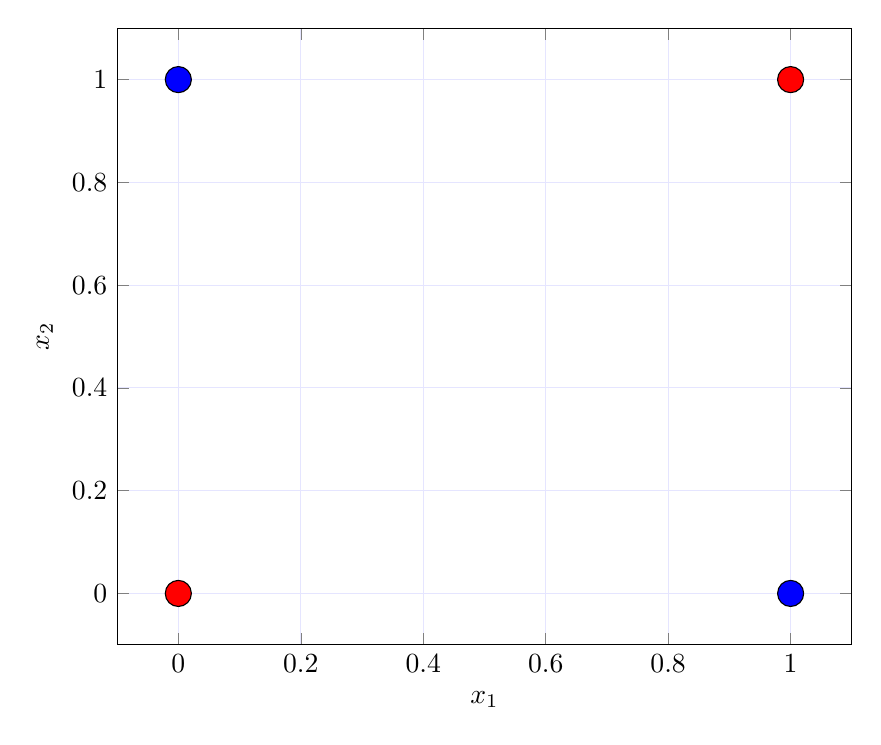
\begin{tikzpicture}
            \begin{axis}[
                width=0.9\linewidth,
                grid=major,
                grid style={line width=.3pt, draw=blue!10},
                major grid style={line width=.3pt, draw=blue!10},
                %minor tick num=2,
                xlabel={$x_1$},
                ylabel={$x_2$},
                xmin=-0.1,
                xmax=1.1,
                ymin=-0.1,
                ymax=1.1
            ]
            \node[draw, circle, fill=red,  radius=0.3cm] at (1, 1) {};
            \node[draw, circle, fill=red,  radius=0.3cm] at (0, 0) {};
            \node[draw, circle, fill=blue, radius=0.3cm] at (1, 0) {};
            \node[draw, circle, fill=blue, radius=0.3cm] at (0, 1) {};
            \end{axis}
            \end{tikzpicture}
        \end{figure}
    \end{column}
    \begin{column}{0.48\textwidth}
        \begin{itemize}
            \item Binary exclusive operator,\\ 
            is $1$ if one operand is $1$, else $0$
            \item Non-linearly separable,\\ 
            logistic regression cannot model problem
            \item \textbf{Idea:} decompose into linear problems
        \end{itemize}
    \end{column}
\end{columns}
\end{frame}

\begin{frame}
\frametitle{XOR-Problem}
\begin{columns}
    \begin{column}{0.32\textwidth}
        \begin{onlyenv}<1->
        \begin{figure}
            \centering
            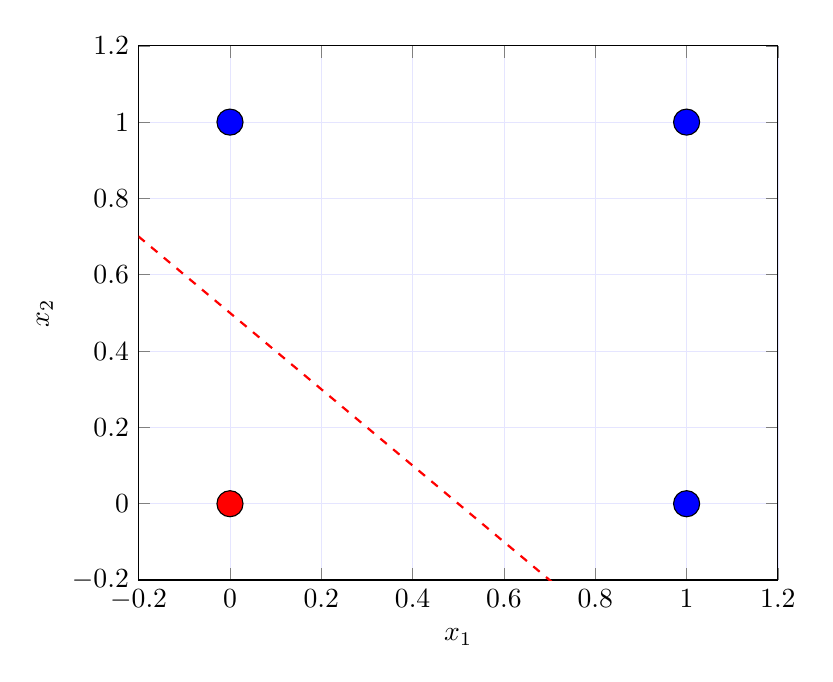
\begin{tikzpicture}
            \begin{axis}[
                width=0.8\linewidth,
                grid=major,
                grid style={line width=.3pt, draw=blue!10},
                major grid style={line width=.3pt, draw=blue!10},
                xlabel={$x_1$},
                ylabel={$x_2$},
                xmin=-0.2,
                xmax=1.2,
                ymin=-0.2,
                ymax=1.2
            ]
            \node[draw, circle, fill=blue, radius=0.05cm] at (1, 1) {};
            \node[draw, circle, fill=red,  radius=0.05cm] at (0, 0) {};
            \node[draw, circle, fill=blue, radius=0.05cm] at (1, 0) {};
            \node[draw, circle, fill=blue, radius=0.05cm] at (0, 1) {};
            \addplot[red, thick, dashed, mark=none] {-x + 0.5};
            \end{axis}
            \end{tikzpicture}
        \end{figure}
        \end{onlyenv}
    \end{column}
    \begin{column}{0.32\textwidth}
        \begin{onlyenv}<2->
        \begin{figure}
            \centering
            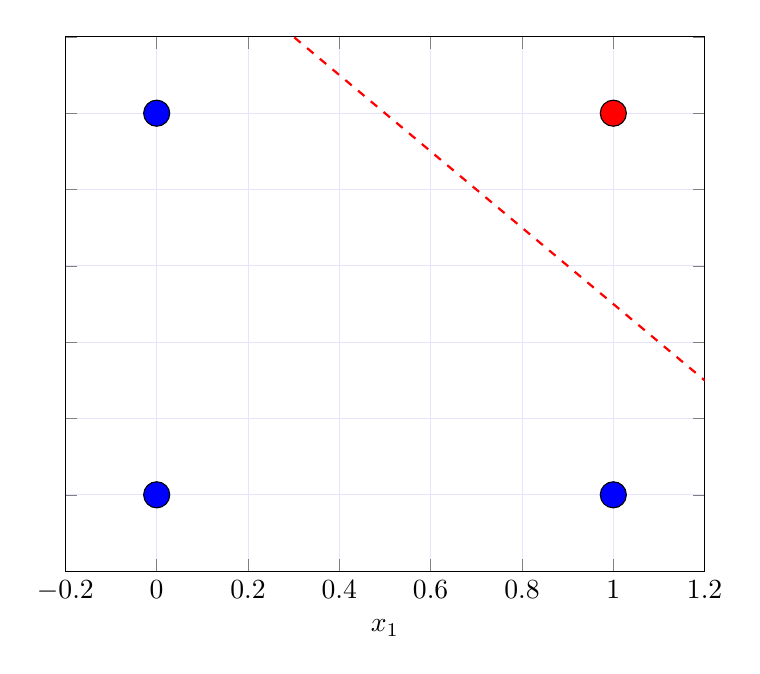
\begin{tikzpicture}
            \begin{axis}[
                width=0.8\linewidth,
                grid=major,
                grid style={line width=.3pt, draw=blue!10},
                major grid style={line width=.3pt, draw=blue!10},
                xlabel={$x_1$},
                yticklabels={,,},
                xmin=-0.2,
                xmax=1.2,
                ymin=-0.2,
                ymax=1.2,
            ]
            \node[draw, circle, fill=red,  radius=0.05cm] at (1, 1) {};
            \node[draw, circle, fill=blue, radius=0.05cm] at (0, 0) {};
            \node[draw, circle, fill=blue, radius=0.05cm] at (1, 0) {};
            \node[draw, circle, fill=blue, radius=0.05cm] at (0, 1) {};
            \addplot[red, thick, dashed, mark=none] {-x + 1.5};
            \end{axis}
            \end{tikzpicture}
        \end{figure}
        \end{onlyenv}
    \end{column}
    \begin{column}{0.32\textwidth}
        \begin{onlyenv}<3->
        \begin{figure}
            \centering
            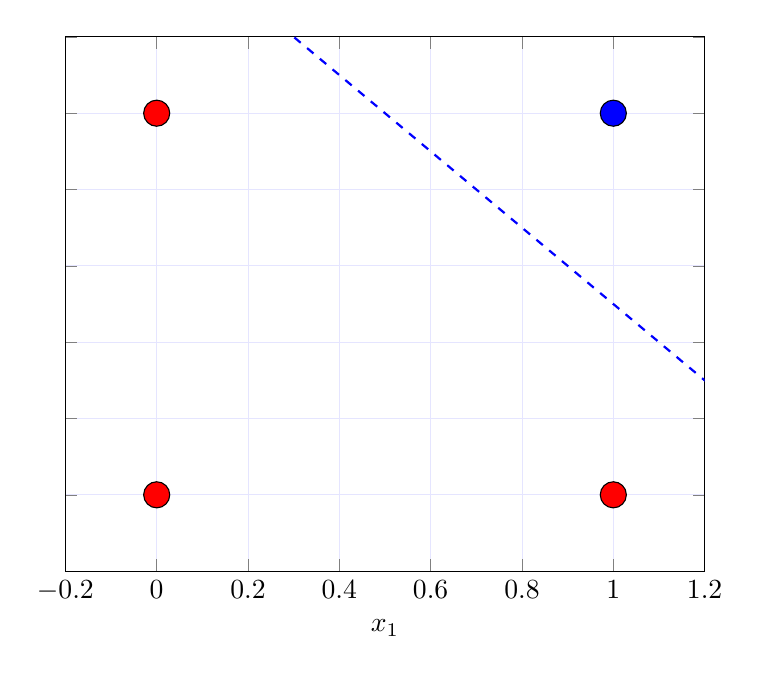
\begin{tikzpicture}
            \begin{axis}[
                width=0.8\linewidth,
                grid=major,
                grid style={line width=.3pt, draw=blue!10},
                major grid style={line width=.3pt, draw=blue!10},
                xlabel={$x_1$},
                yticklabels={,,},
                xmin=-0.2,
                xmax=1.2,
                ymin=-0.2,
                ymax=1.2,
            ]
            \node[draw, circle, fill=blue, radius=0.05cm] at (1, 1) {};
            \node[draw, circle, fill=red,  radius=0.05cm] at (0, 0) {};
            \node[draw, circle, fill=red,  radius=0.05cm] at (1, 0) {};
            \node[draw, circle, fill=red,  radius=0.05cm] at (0, 1) {};
            \addplot[blue, thick, dashed, mark=none] {-x + 1.5};
            \end{axis}
            \end{tikzpicture}
        \end{figure}
        \end{onlyenv}
    \end{column}
\end{columns}
\bigskip
\begin{columns}
    \begin{column}{0.32\textwidth}
        \centering
        \begin{onlyenv}<1->
        \textbf{OR-gate}\\
        \medskip
        $h_1=sig(2x_1 + 2x_2 + 1)$
    \end{onlyenv}
    \end{column}
    \begin{column}{0.32\textwidth}
        \centering
        \begin{onlyenv}<2->
        \textbf{NAND-gate}\\
        \medskip
        $h_2=sig(-2x_1 -2x_2 - 1.5)$
    \end{onlyenv}
    \end{column}
    \begin{column}{0.32\textwidth}
        \centering
        \begin{onlyenv}<3->
        \textbf{AND-gate}\\
        \medskip
        $\hat{y}=sig(2h_1 +2h_2 + 3)$
        \end{onlyenv}
    \end{column}
\end{columns}
\end{frame}

\begin{frame}
\frametitle{Fully-connected Neural Network}

\begin{columns}
    \begin{column}{0.48\textwidth}
        \begin{figure}
            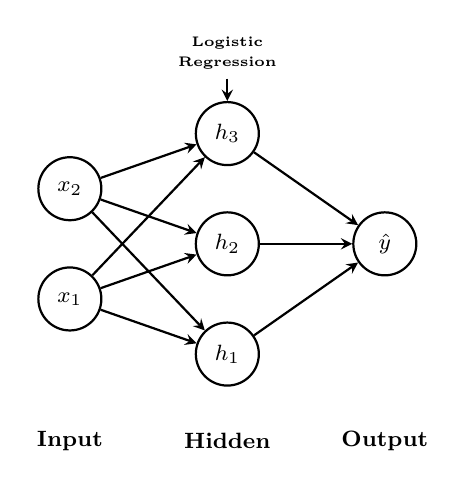
\begin{tikzpicture}
            \node[draw, circle, thick, minimum size=0.8cm] (input1) at (-2,-0.7) {\footnotesize$x_1$};
            \node[draw, circle, thick, minimum size=0.8cm] (input2) at (-2, 0.7) {\footnotesize$x_2$};
            
            \node[draw, circle, thick, minimum size=0.8cm] (hidden1) at (0,-1.4) {\footnotesize$h_1$};
            \node[draw, circle, thick, minimum size=0.8cm] (hidden2) at (0, 0)   {\footnotesize$h_2$};
            \node[draw, circle, thick, minimum size=0.8cm] (hidden3) at (0, 1.4) {\footnotesize$h_3$};
            
            \node[draw, circle, thick, minimum size=0.8cm] (output) at (2, 0) {\footnotesize$\hat{y}$};
            
            \draw[->, >=stealth, thick] (input1)--(hidden1);
            \draw[->, >=stealth, thick] (input1)--(hidden2);
            \draw[->, >=stealth, thick] (input1)--(hidden3);
            
            \draw[->, >=stealth, thick] (input2)--(hidden1);
            \draw[->, >=stealth, thick] (input2)--(hidden2);
            \draw[->, >=stealth, thick] (input2)--(hidden3);
            
            \draw[->, >=stealth, thick] (hidden1)--(output);
            \draw[->, >=stealth, thick] (hidden2)--(output);
            \draw[->, >=stealth, thick] (hidden3)--(output);
            
            \node at (-2, -2.5) {\footnotesize \textbf{Input}};
            \node at ( 0, -2.5) {\footnotesize \textbf{Hidden}};
            \node at ( 2, -2.5) {\footnotesize \textbf{Output}};
            
            \node[align=center] at (0, 2.55) {\textbf{\tiny Logistic}};
            \node[align=center] (reg) at (0, 2.3) {\textbf{\tiny Regression}};
            \draw[->, >=stealth, thick] (reg)--(hidden3);
            \end{tikzpicture}
        \end{figure}
    \end{column}
    \begin{column}{0.48\textwidth}
        \begin{itemize}
            \item Inspired by biological neural network
            \item A \textbf{neuron} is a logistic regression
            \item Neurons are arranged in \textbf{layers}
            \item Layers are \textbf{fully-connected} with subsequent layer, also called \textbf{Dense}
            \item \textbf{Width:} neuron count
            \item \textbf{Depth:} layer count
        \end{itemize}
    \end{column}
\end{columns}
\end{frame}

\begin{frame}
\frametitle{Universal Approximation Theorem}

\uncover<1->{
A feed-forward neural network with a linear output and at least one hidden layer can approximate any reasonable function to arbitrary precision with a finite number of nodes.
}
\vspace{0.5cm}
\begin{itemize}
    \item<2-> \textbf{Good News}
    \begin{itemize}
        \item Networks can perform highly complex tasks
        \item All necessary ingredients available
    \end{itemize}
    \item<3-> \textbf{Bad News}
    \begin{itemize}
        \item Does not specify number of necessary nodes
        \item No remarks on neuron connectivity
    \end{itemize}
\end{itemize}
\end{frame}

\subsection{Backpropagation}
\label{subsec:backpropagation}

\subsection{Multi-class Classification}
\label{subsec:multi-class-classification}

\begin{frame}
\frametitle{Multi-class Classification}

\begin{itemize}
    \item \textbf{One-hot class encoding:} encode classes as sparse vectors \\
    $y=(y_1, y_2, ..., y_c)$, only one is active, e.g. class $2\rightarrow (0, 1, ..., 0)$
    \item \textbf{Softmax output activation:} $\hat{y}=softmax(z)=\frac{e^{z_{j}}}{\sum_{j}e^{z_{j}}}$ for $j=1...c$\\
    achieve joint-probability of $1$, normalize across model outputs $z$
    \item \textbf{Cross-entropy loss:} convex-function $J(w)=\frac{1}{n}\sum_{i=1}^{n}\sum_{j}^{c}y_{i,j}\log\hat{y}_{i,j}$\\
    maximum likelihood principle
\end{itemize}
\end{frame}

\subsection{Addition Components}
\label{subsec:more-components}

\begin{frame}
\frametitle{Activation Functions}

\begin{itemize}
    \item Activation functions $a(x)$ introduce \textbf{non-linearity}, e.g. sigmoid function
    \item Other non-linear choices, e.g. $tanh(x)$, $relu(x)=max(0,x)$, etc.
    \item Better computational properties, e.g. avoid \textbf{vanishing gradient}
\end{itemize}
\vspace{-0.5cm}
\begin{figure}
    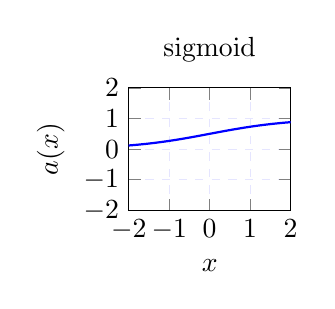
\begin{tikzpicture}
    \begin{axis}[
        title=sigmoid,
        width=0.3\linewidth, 
        grid=major,
        grid style={dashed, line width=.3pt, draw=blue!10},
        major grid style={line width=.3pt, draw=blue!10},
        xlabel={$x$},
        ylabel={$a(x)$},
        xmin=-2,
        xmax=2,
        ymin=-2,
        ymax=2
    ]
    \addplot [blue, thick, mark=none, smooth, samples=50] {1/(1+e^(-x))};
    \end{axis} 
    \end{tikzpicture}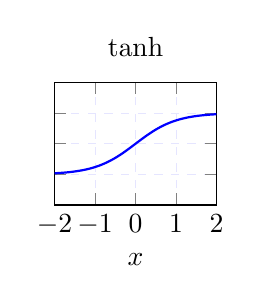
\begin{tikzpicture}
    \begin{axis}[
        title=tanh,
        width=0.3\linewidth, 
        grid=major,
        grid style={dashed, line width=.3pt, draw=blue!10},
        major grid style={line width=.3pt, draw=blue!10},
        yticklabels={,,},
        xlabel={$x$},
        xmin=-2,
        xmax=2,
        ymin=-2,
        ymax=2
    ]
    \addplot [blue, thick, mark=none, smooth, samples=50] {tanh(x)};
    \end{axis}
    \end{tikzpicture}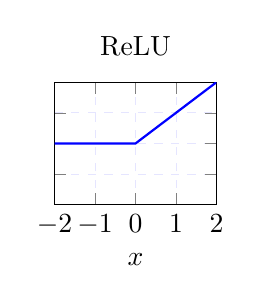
\begin{tikzpicture}
    \begin{axis}[
        title=ReLU,
        width=0.3\linewidth, 
        grid=major,
        grid style={dashed, line width=.3pt, draw=blue!10},
        major grid style={line width=.3pt, draw=blue!10},
        yticklabels={,,},
        xlabel={$x$},
        xmin=-2,
        xmax=2,
        ymin=-2,
        ymax=2
    ]
    \addplot [blue, thick, mark=none, domain=-3:3] {max(0, x)};
    \end{axis}
    \end{tikzpicture}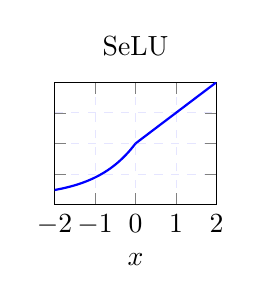
\begin{tikzpicture}
    \begin{axis}[
        title=SeLU,
        width=0.3\linewidth, 
        grid=major,
        grid style={dashed, line width=.3pt, draw=blue!10},
        major grid style={line width=.3pt, draw=blue!10},
        yticklabels={,,},
        xlabel={$x$},
        xmin=-2,
        xmax=2,
        ymin=-2,
        ymax=2
    ]
    \addplot [blue, thick, mark=none, smooth, samples=50, domain=-3:0]{1.0507 * 1.6732 * (e^x - 1)};
    \addplot [blue, thick, mark=none, smooth, samples=50, domain=0:3]{x};
    \end{axis}
    \end{tikzpicture}
\end{figure}
\end{frame}

\subsection{Generalization}
\label{subsec:generalization}

\begin{frame}
\frametitle{Over- and Underfitting}
\end{frame}

\begin{frame}
\frametitle{Over- and Underfitting}

\begin{columns}
    \begin{column}{0.48\textwidth}
        \begin{figure}
            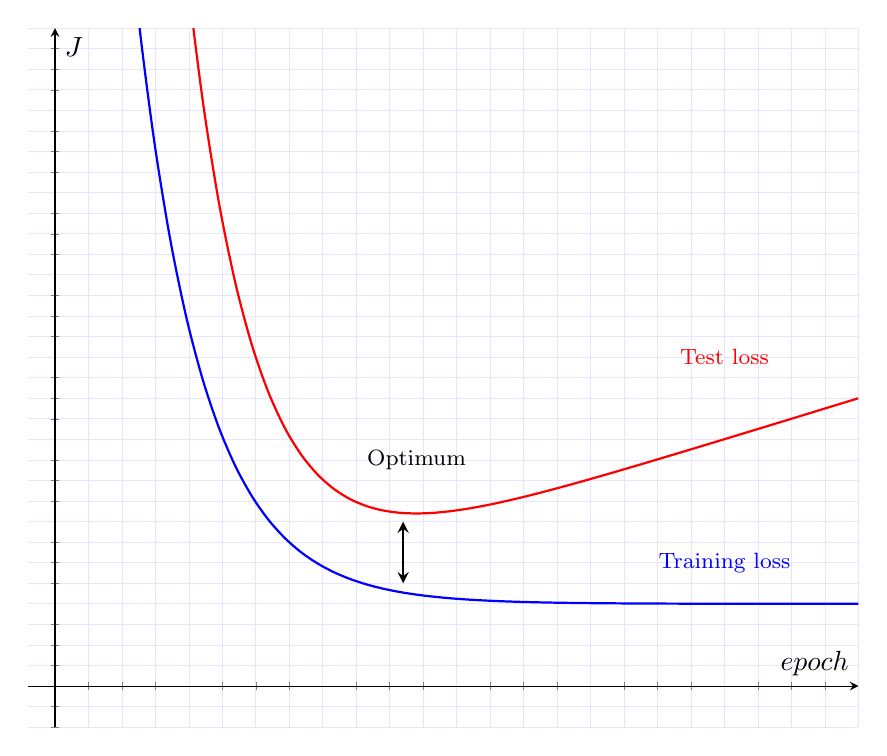
\begin{tikzpicture}
            \begin{axis}[
                width=\linewidth, 
                grid=both,
                grid style={line width=.3pt, draw=blue!10},
                major grid style={line width=.3pt, draw=blue!10},
                minor tick num=3,
                xlabel={$epoch$},
                ylabel={$J$}, 
                ticks=none,
                axis x line=center,
                axis y line=center,
                xmin=-0.1,
                xmax=3.0,
                ymin=-0.1,
                ymax=1.6
            ]
            % domain=0.25:2.75
            \addplot [red, thick, mark=none, smooth, samples=50, domain=0:3] {e^(-4*(x-0.6)) + 0.1 + 0.2*x};
            \addplot [blue, thick, mark=none, smooth, samples=50, domain=0:3] {e^(-4*(x-0.4)) + 0.2};
            \draw[<->, black, >=stealth, thick] (axis cs:1.3,0.25)--(axis cs:1.3,0.4);
            \node at (axis cs:2.5,0.8) [red]  {\footnotesize Test loss};
            \node at (axis cs:2.5,0.3) [blue] {\footnotesize Training loss};
            \node at (axis cs:1.35,0.55) [black] {\footnotesize Optimum};
            \end{axis} 
            \end{tikzpicture}
        \end{figure}
    \end{column}
    \begin{column}{0.48\textwidth}
        \begin{itemize}
            \item Separate monitoring of training and test loss during training
            \item Training loss will decrease indefinitely\\ $J\rightarrow 0$, \textbf{memorization effect}
            \item \textbf{Test loss minimum} is optimal
        \end{itemize}
    \end{column}
\end{columns}
\end{frame}

\begin{frame}
\frametitle{Regularization}
\end{frame}

\begin{frame}
\frametitle{Dropout}

\begin{itemize}
    \item Randomly turn of neurons and connection, e.g. $p(drop)=0.5$
    \item Equivalent to network regularization (proof omitted)
\end{itemize}

\begin{columns}
    \begin{column}{0.48\textwidth}
        \begin{figure}
            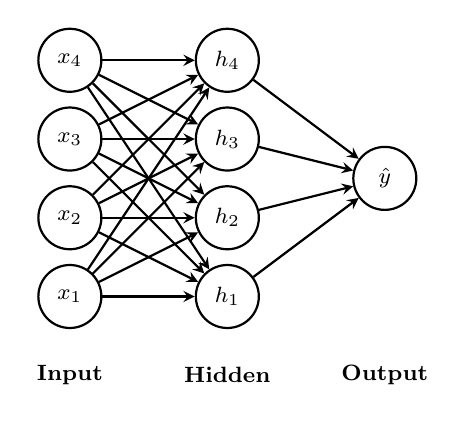
\begin{tikzpicture}
            \node[draw, circle, thick, minimum size=0.8cm] (input1) at (-2,-1.5) {\footnotesize$x_1$};
            \node[draw, circle, thick, minimum size=0.8cm] (input2) at (-2,-0.5) {\footnotesize$x_2$};
            \node[draw, circle, thick, minimum size=0.8cm] (input3) at (-2, 0.5) {\footnotesize$x_3$};
            \node[draw, circle, thick, minimum size=0.8cm] (input4) at (-2, 1.5) {\footnotesize$x_4$};
            
            \node[draw, circle, thick, minimum size=0.8cm] (hidden1) at (0,-1.5) {\footnotesize$h_1$};
            \node[draw, circle, thick, minimum size=0.8cm] (hidden2) at (0,-0.5) {\footnotesize$h_2$};
            \node[draw, circle, thick, minimum size=0.8cm] (hidden3) at (0, 0.5) {\footnotesize$h_3$};
            \node[draw, circle, thick, minimum size=0.8cm] (hidden4) at (0, 1.5) {\footnotesize$h_4$};
            
            \node[draw, circle, thick, minimum size=0.8cm] (output) at (2, 0) {\footnotesize$\hat{y}$};
            
            \draw[->, >=stealth, thick] (input1)--(hidden1);
            \draw[->, >=stealth, thick] (input1)--(hidden2);
            \draw[->, >=stealth, thick] (input1)--(hidden3);
            \draw[->, >=stealth, thick] (input1)--(hidden4);
            
            \draw[->, >=stealth, thick] (input2)--(hidden1);
            \draw[->, >=stealth, thick] (input2)--(hidden2);
            \draw[->, >=stealth, thick] (input2)--(hidden3);
            \draw[->, >=stealth, thick] (input2)--(hidden4);
            
            \draw[->, >=stealth, thick] (input3)--(hidden1);
            \draw[->, >=stealth, thick] (input3)--(hidden2);
            \draw[->, >=stealth, thick] (input3)--(hidden3);
            \draw[->, >=stealth, thick] (input3)--(hidden4);
            
            \draw[->, >=stealth, thick] (input4)--(hidden1);
            \draw[->, >=stealth, thick] (input4)--(hidden2);
            \draw[->, >=stealth, thick] (input4)--(hidden3);
            \draw[->, >=stealth, thick] (input4)--(hidden4);
            
            \draw[->, >=stealth, thick] (hidden1)--(output);
            \draw[->, >=stealth, thick] (hidden2)--(output);
            \draw[->, >=stealth, thick] (hidden3)--(output);
            \draw[->, >=stealth, thick] (hidden4)--(output);
            
            \node at (-2, -2.5) {\footnotesize \textbf{Input}};
            \node at ( 0, -2.5) {\footnotesize \textbf{Hidden}};
            \node at ( 2, -2.5) {\footnotesize \textbf{Output}};
            \end{tikzpicture}
        \end{figure}
    \end{column}
    \begin{column}{0.48\textwidth}
        \begin{figure}
            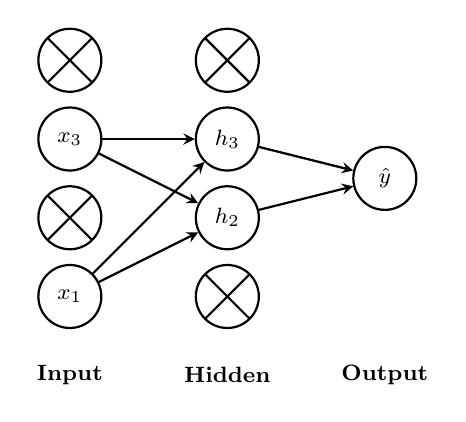
\begin{tikzpicture}
            \node[draw, circle, thick, minimum size=0.8cm] (input1) at (-2,-1.5) {\footnotesize$x_1$};
            \node[draw, cross, circle, thick, minimum size=0.8cm] (input2) at (-2,-0.5) {};
            \node[draw, circle, thick, minimum size=0.8cm] (input3) at (-2, 0.5) {\footnotesize$x_3$};
            \node[draw, cross, circle, thick, minimum size=0.8cm] (input4) at (-2, 1.5) {};
            
            \node[draw, cross, circle, thick, minimum size=0.8cm] (hidden1) at (0,-1.5) {};
            \node[draw, circle, thick, minimum size=0.8cm] (hidden2) at (0,-0.5) {\footnotesize$h_2$};
            \node[draw, circle, thick, minimum size=0.8cm] (hidden3) at (0, 0.5) {\footnotesize$h_3$};
            \node[draw, cross, circle, thick, minimum size=0.8cm] (hidden4) at (0, 1.5) {};
            
            \node[draw, circle, thick, minimum size=0.8cm] (output) at (2, 0) {\footnotesize$\hat{y}$};
            
            \draw[->, >=stealth, thick] (input1)--(hidden2);
            \draw[->, >=stealth, thick] (input1)--(hidden3);
            
            \draw[->, >=stealth, thick] (input3)--(hidden2);
            \draw[->, >=stealth, thick] (input3)--(hidden3);
            
            \draw[->, >=stealth, thick] (hidden2)--(output);
            \draw[->, >=stealth, thick] (hidden3)--(output);
            
            \node at (-2, -2.5) {\footnotesize \textbf{Input}};
            \node at ( 0, -2.5) {\footnotesize \textbf{Hidden}};
            \node at ( 2, -2.5) {\footnotesize \textbf{Output}};
            \end{tikzpicture}
        \end{figure}
    \end{column}
\end{columns}
\end{frame}

\subsection{Exercise: MNIST FNN}
\label{subsec:exercise-fnn}

\begin{frame}
    \frametitle{Exercise: FNN MNIST Image Classification}
    
    \begin{figure}
        \centering
        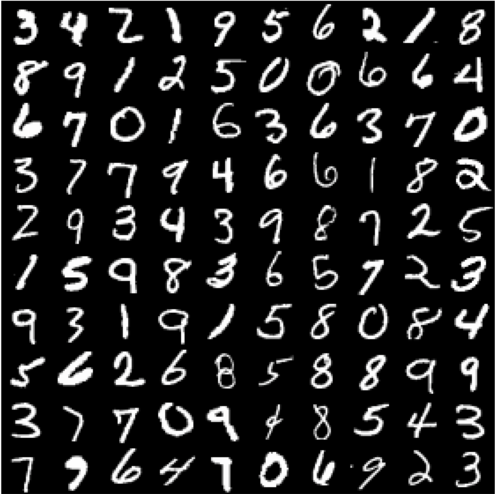
\includegraphics[width=0.4\linewidth]{mnist.png}
    \end{figure}
\end{frame}

\section{Convolutional Neural Networks}
\label{sec:convolutional-neural-networks}

\subsection{Deep Learning}
\label{subsec:deep-learning}

\subsection{Discrete Convolution}
\label{subsec:discrete-convolution}

\begin{frame}
    \frametitle{Discrete Convolution}
    \begin{figure}
        \centering
        \multiinclude[<+->][format=png, graphics={width=0.8\linewidth}]{convolution}
        \imageright{Machine Learning Guru}
    \end{figure}
\end{frame}

\begin{frame}
\frametitle{Pooling}
\end{frame}

\begin{frame}
\frametitle{Optimizers}
\end{frame}

\begin{frame}
\frametitle{Hyperparameter Optimization}
\end{frame}

\subsection{Network Architectures}
\label{subsec:network-architectures}

\begin{frame}
\frametitle{Inception}
\end{frame}

\begin{frame}
\frametitle{ResNet}
\end{frame}

\subsection{Exercise: MNIST CNN}
\label{subsec:cnn-exercise}

\begin{frame}
\frametitle{Exercise: FNN MNIST Image Classification}

\begin{figure}
    \centering
    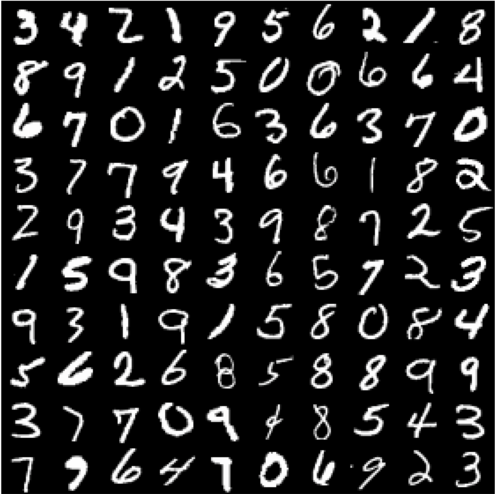
\includegraphics[width=0.4\linewidth]{mnist.png}
\end{figure}
\end{frame}

\section{Regression}
\label{sec:regression}

\subsection{Exercise: Abalone}
\label{subsec:regression-exercise}

\begin{frame}
    \frametitle{Exercise: Abalone Age Regression Analysis}
    \begin{figure}
        \centering
        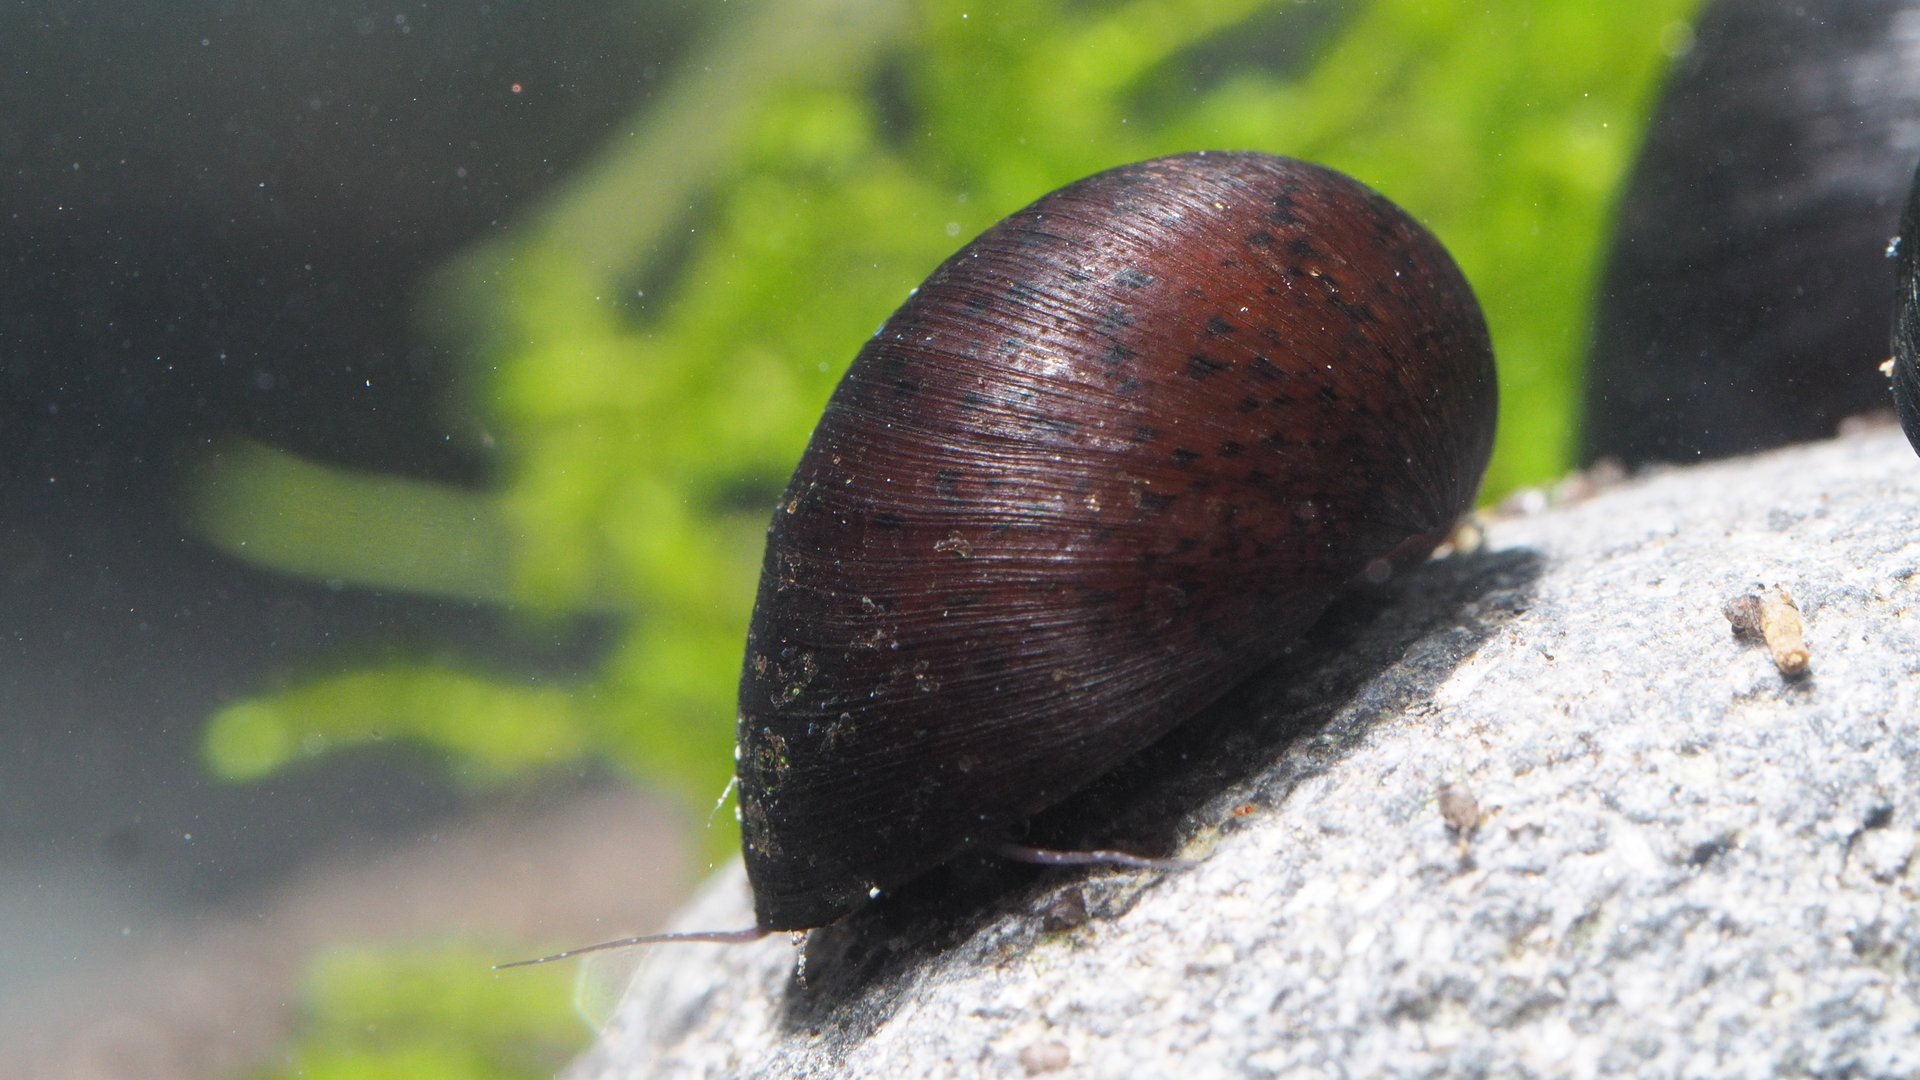
\includegraphics[width=0.7\linewidth]{abalone.jpg}
        \imageright{Garnelaxia}
    \end{figure}
\end{frame}

\section{Summary}
\label{sec:summary}

\begin{frame}
\frametitle{Summary}

\begin{itemize}
    \item Supervised machine learning
    \begin{itemize}
        \item Logistic regression
        \item (Convolutional) neural networks
    \end{itemize}
\end{itemize}
\end{frame}

\begin{frame}
\frametitle{Open Topics}
\end{frame}

\begin{frame}
\frametitle{Acknowledgment}

\begin{columns}
    \begin{column}{0.48\textwidth}
        \begin{itemize}
            \item \textbf{Eileen Kühn}
            \begin{itemize}
                \item GridKa School organization
                \item Paperwork
            \end{itemize}
            \item \textbf{Oskar Taubert}
            \begin{itemize}
                \item Assignment preparation
                \item Exercise supervision
            \end{itemize}
            \item \textbf{Andreas Herten}
            \begin{itemize}
                \item Access to JURON
                \item Technical support
            \end{itemize}
        \end{itemize}
    \end{column}

    \begin{column}{0.48\textwidth}
        \begin{figure}
            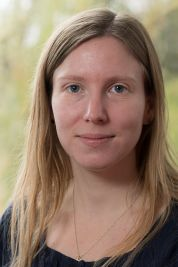
\includegraphics[width=0.25\linewidth]{eileen.jpg}\quad 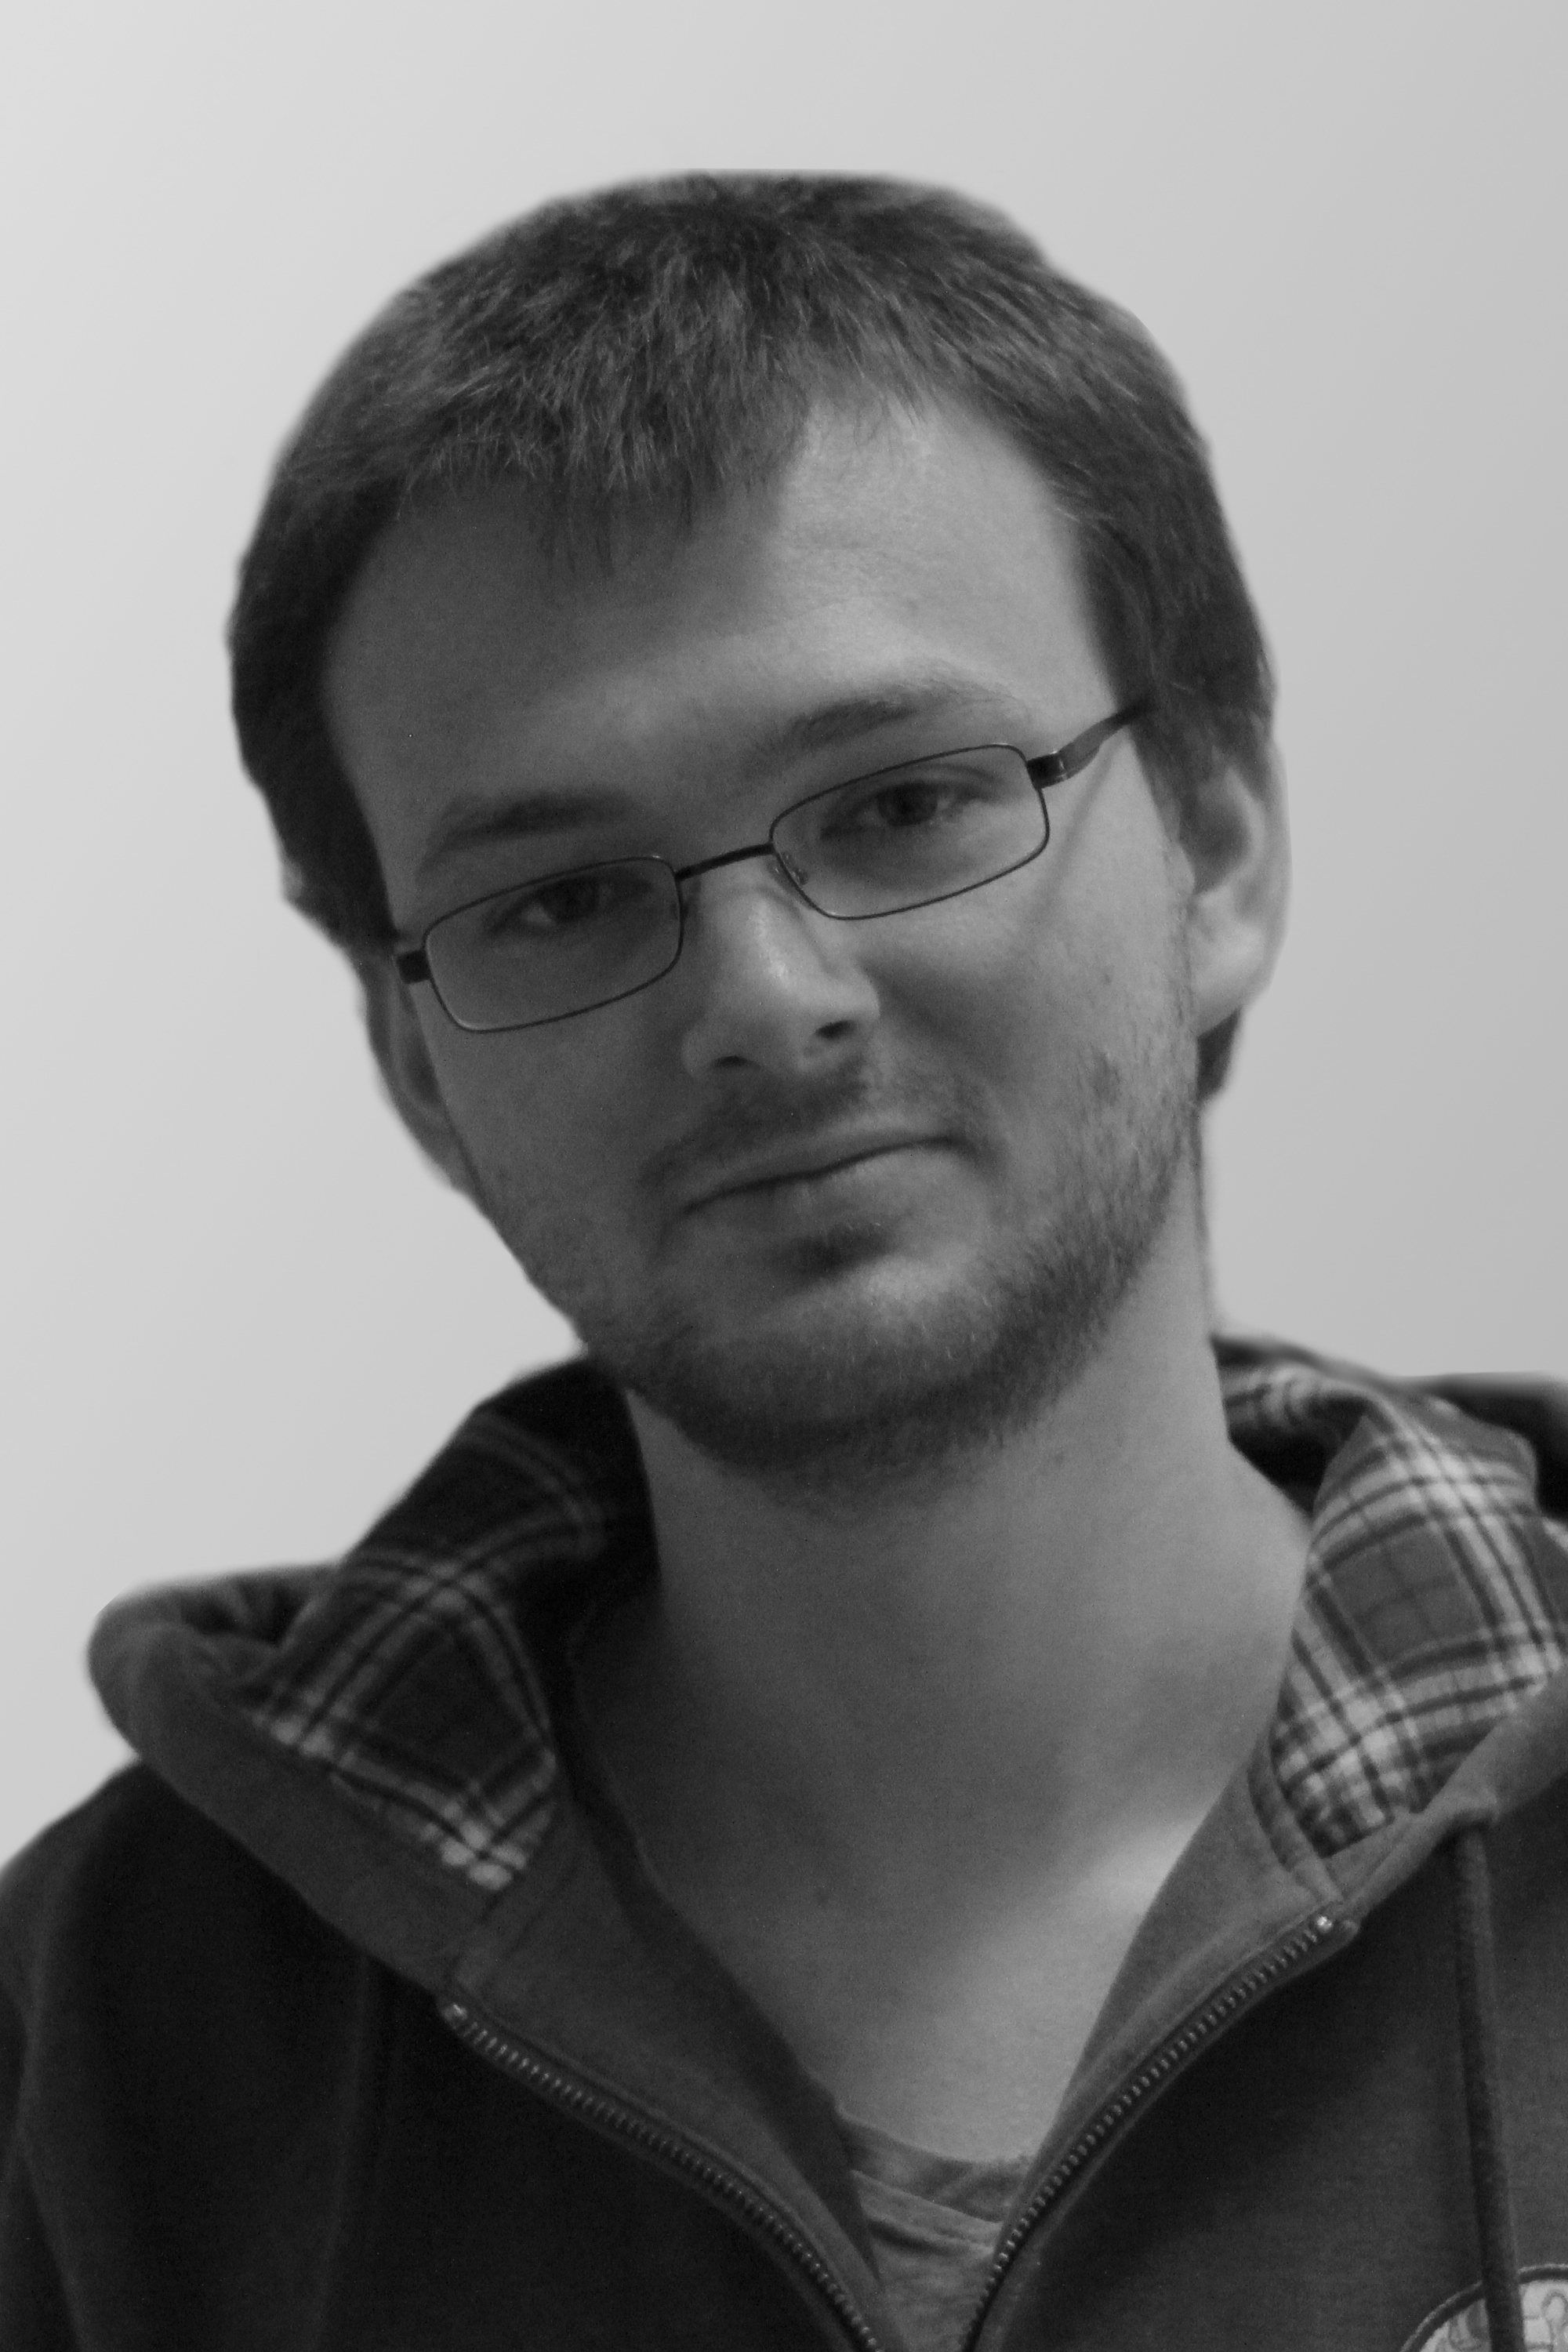
\includegraphics[width=0.25\linewidth]{oskar.jpg} \\\medskip
            
            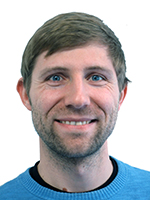
\includegraphics[width=0.25\linewidth]{andreas.jpg}\quad 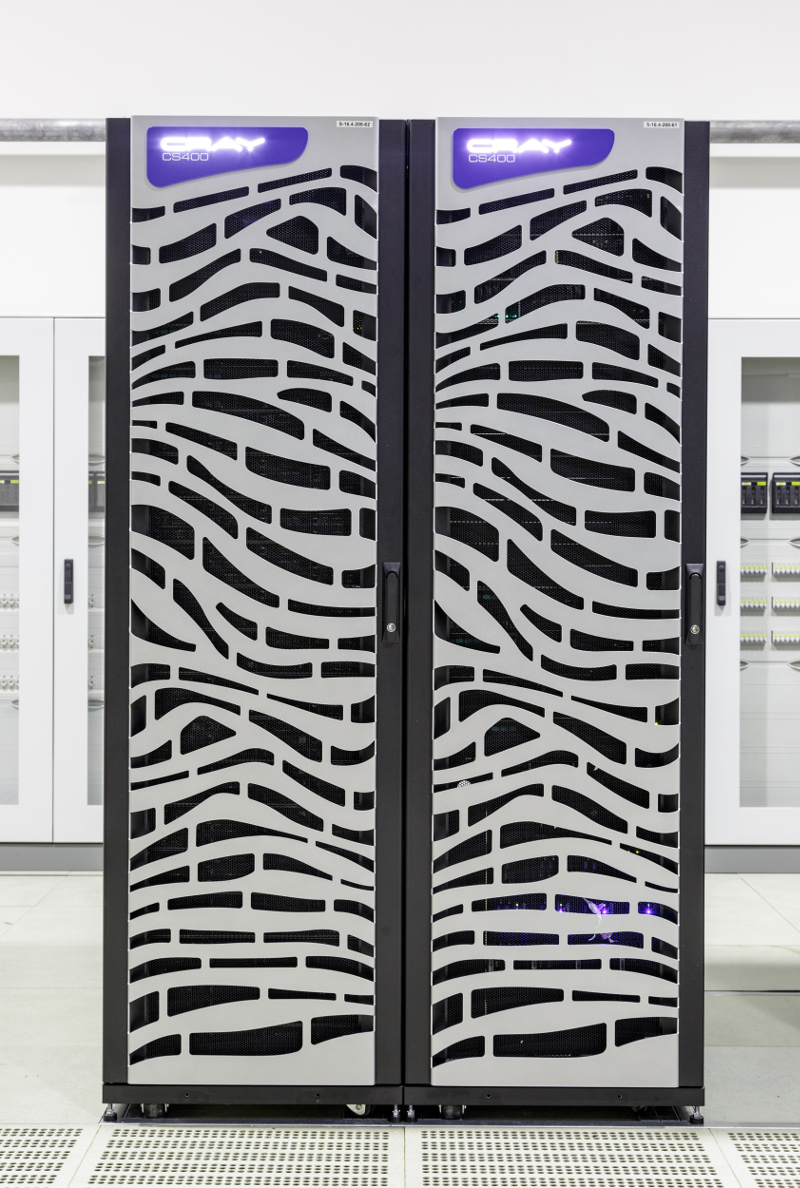
\includegraphics[width=0.25\linewidth]{juron.jpg} \\
        \end{figure}
    \end{column}
\end{columns}
\end{frame}

\end{document}
